% Standalone Supplementary Information root for the Nature Food submission.
\documentclass[pdflatex,sn-nature]{sn-jnl}

\usepackage{amsmath,amssymb,amsfonts}
\usepackage{booktabs}
\usepackage{graphicx}

\raggedbottom

\begin{document}

\title{Supplementary Information for: Bounded attribute-level calibration for microbiome-informed nutrient profiling}
\maketitle

\setcounter{section}{0}
\setcounter{subsection}{0}
\setcounter{equation}{0}
\setcounter{figure}{0}
\setcounter{table}{0}
\renewcommand{\thesection}{S\arabic{section}}
\renewcommand{\thesubsection}{\thesection.\arabic{subsection}}
\renewcommand{\theequation}{S\arabic{equation}}
\renewcommand{\thefigure}{S\arabic{figure}}
\renewcommand{\thetable}{S\arabic{table}}

\section{Supplementary Methods}

\subsection*{Locked computational specification and provenance}

The frozen specification is \texttt{attribute-gmnps-v1}. Its primary method is
\texttt{attribute\_recomposition}, its primary mapping is
\texttt{expert\_reviewed\_attribute\_mapping\_v1}, and its recomposition rule is
\texttt{native\_domain\_fixed\_residual\_v1}. Expert review refers only to
nutrient-channel content. The numerical allocation weights are author-specified.
Mapping roles, allocation weights,
attribute rules, temperatures, cap modes, domain membership and score centring
were locked before outcome access. The six recomputed domains are
\texttt{nutrient\_ratios}, \texttt{vitamins}, \texttt{minerals},
\texttt{specific\_lipids}, \texttt{fiber\_and\_protein}, and
\texttt{phytochemicals}. The complete versioned attribute registry and
nutrient-to-attribute mapping, including rules, roles, component policies and
allocation weights, are supplied as Supplementary Data 1 in
\texttt{supplementary\_data\_1\_attribute\_mapping\_table.csv}.

An eligible production run must bind the trusted release-registry snapshot, one approved artifact entry, immutable source bytes and parsed-content fingerprints, release labels, food and participant linkage and units, nutrient/exposure basis, development and beta inputs, configuration digests, and source-code digests. The current registry has no approved production
artifact, so no empirical production-food result is authorized and no
placeholder production instance was created.

\subsection*{Food Compass attribute scoring}

Food Compass 2.0 contains 54 conceptual attributes represented by 56
operational rows because fruits and non-starchy vegetables each have separate
dried and non-dried rows. In the locked USDA-oriented specification, 54 rows
are active. For an ordinary linear rule with exposure \(x\), targets
\((t_0,t_1)\) and native points \((p_0,p_1)\), points are calculated as
\[
p(x)=\operatorname{clip}\!\left[
p_0+\frac{x-t_0}{t_1-t_0}(p_1-p_0),
\min(p_0,p_1),\max(p_0,p_1)\right].
\]
Negative linear exposures are invalid. Ratio rules use the same interpolation
on \(\log(x)\) and require \(x>0\). Added-sugar cut points are exactly 2.5, 5,
10, 15, 20, 30, 40, 50 and 60 percent energy, with 0 points at zero exposure
and -1 through -10 thereafter. Binary additive attributes use presence/absence
points, and NOVA class is interpolated through \((1,10)\), \((2,7.5)\),
\((3,5)\), and \((4,-10)\). The primary nitrite rule is the published
50\%-energy footnote interpretation; the conflicting 25\% table value is
retained only as a named sensitivity setting.

Composition exposures are expressed per 100 kcal unless the rule explicitly
uses percentage energy, a ratio, binary presence or NOVA class. The three ratio
gates are fixed: unsaturated-to-saturated fat requires at least 10\% energy from
fat; fibre-to-carbohydrate requires at least 10\% energy from carbohydrate; and
potassium-to-sodium requires at least 10 mg of both potassium and sodium per
100 kcal. A failed gate produces the canonical \texttt{NOT\_CALCULATED} value
and removes the attribute from the active domain denominator. For dairy foods,
the effective weight of unsaturated-to-saturated fat is 0.5; its weight is 1.0
for non-dairy foods.

For calculated attributes \(a\) in domain \(A\), ordinary domain aggregation is
\[
\overline p_A=\frac{\sum_{a\in A}p_av_a}{\sum_{a\in A}v_a},
\]
where \(v_a\) is the effective attribute weight. The food-ingredients domain is
a weighted sum. Vitamins and minerals retain the five largest absolute native
points, specific lipids retain the three largest, and ties follow immutable
registry order. Specific-lipid and phytochemical domain contributions each
receive their published factor of 0.5.

\subsection*{Unavailable values and missingness}

Iodine and trans-fat percentage of energy are inactive because the source
specification records them as unavailable. They are neither imputed nor treated
as zero. When local 18:3 cannot be verified as alpha-linolenic acid, the
alpha-linolenic-acid point is retained as a fixed baseline attribute inside the
recomputed specific-lipids domain. Total flavonoids are handled analogously when
the separate flavonoid source is absent. Food-ingredient attributes require
their food-pattern-equivalent source, additives require ingredient or additive
records, and processing attributes require processing or recipe records. Total
sugar cannot replace added sugar, and a rounded NOVA category cannot replace an
energy-weighted mixed-dish value. Missing requirements therefore produce an
unavailable or fixed-baseline state rather than zero filling.

\subsection*{Development-only beta normalization}

The upstream microbiome interface begins with a centred log-ratio genus matrix
\(M\). A sparse L1-regularized logistic regression \(H\) is fitted in the development
set to distinguish available healthy from non-healthy metadata labels. Duplicate
or contradictory health labels are excluded from fitting. Genus means and
scales are estimated in development data; missing genera in later scoring data
are aligned to the fitted genus order and filled with the corresponding
development mean. No additional cross-cohort batch correction is performed by
this module, so harmonized taxonomic processing and explicit cohort/batch
sensitivity checks are prerequisites for empirical evaluation.

For nutrient \(n\), the nutrient-to-genus bridge is aligned to the fitted genera.
Each bridge row is oriented by the sign and square root of the absolute fitted
health-index coefficient and by the prespecified nutrient-channel direction,
row-centred, L2-normalized to the locked norm of 2.0 and multiplied by its
channel weight to obtain \(P_n\). With the locked perturbation dose
\(\delta=0.25\), the raw individual
input is
\[
b_{in}=\frac{H(M_i+\delta P_n)-H(M_i-\delta P_n)}{2\delta}.
\]
The health index is evaluated on its logit scale. Values are clipped to the
locked absolute numerical limit of 25 only after finite differencing. Health labels define the
development index and are excluded from downstream endpoint adjudication. Any
endpoint assessment must keep health-index fitting, normalization and endpoint
evaluation in disjoint subject or family components.

For raw calibration input \(b_{in}\), development median \(m_n\) and nutrient
\(n\), the first positive scale is selected in this order:
\[
s_n=
\begin{cases}
1.4826\,\operatorname{median}_d|b_{dn}-m_n|, & \text{if positive},\\
(q_{75,n}-q_{25,n})/1.349, & \text{otherwise if positive},\\
\operatorname{sd}_{d,\mathrm{ddof}=0}(b_{dn}), & \text{otherwise if positive},\\
1, & \text{otherwise}.
\end{cases}
\]
The normalized value is
\[
z_{in}=\tanh\!\left(\frac{b_{in}-m_n}{2s_n}\right).
\]
The nutrient order, medians, scales, scale-source methods, development fit
count, SHA-256 of sorted development identifiers, method version and
normalization temperature are immutable normalization state. Held-out or later
scoring participants are transformed with this state and are never appended to
the development fit.

\subsection*{Nutrient-to-attribute response construction}

For normalized exposure \(e_{jna}\), mapping from nutrient \(n\) to native
attribute \(a\), and allocation \(w_{na}\), the uncapped response is
\[
r_{ija}=\sum_{n\mapsto a}z_{in}e_{jna}w_{na}.
\]
Allocations from one nutrient sum exactly to one. Direct exposures are divided
by the largest non-zero absolute published target. Composite components are
divided by their target only after a verified non-zero total. Folate-food and
retinol component fractions preserve the component exposure algebraically while
requiring the corresponding dietary-folate-equivalent or retinol-activity-
equivalent total. The ratio-side policies contribute fibre divided by 9.5 when
the carbohydrate gate passes, potassium divided by 1,175 when both ratio sides
pass, and the negative saturated-fat fraction of saturated plus mono- and
polyunsaturated fat when the fat gate passes. Carbohydrate is inactive in the
primary mapping and appears only in its named sensitivity proxy.

\subsection*{Native point movement and fixed-residual recomposition}

For native range \([l_a,h_a]\), primary fraction \(c=0.20\) and response
temperature 2.0,
\[
\Delta p_{ija}=c(h_a-l_a)\tanh(r_{ija}/2),\qquad
p_{ija}=\operatorname{clip}(p_{ja}+\Delta p_{ija},l_a,h_a).
\]
The 20\% fraction, response temperature and final 12-point cap are
prespecified regularization constants; they are not biologically estimated
thresholds. The 10\% and 30\% attribute fractions and 8- and 15-point final caps
were reserved for future sensitivity analyses and were not evaluated in the
present evidence package.
A baseline \texttt{NOT\_CALCULATED} value remains
\texttt{NOT\_CALCULATED}; attributes outside reviewed targets have zero
response and zero movement.

The official 1-to-100 Food Compass score \(F\) and unscaled value \(U\) are
related by
\[
F(U)=1+\frac{99\{\operatorname{clip}(U,-12.1,35.0)+12.1\}}{47.1},
\qquad
U(F)=-12.1+\frac{47.1(F-1)}{99}.
\]
For food \(j\), the baseline contributions of selected recomputed domains are
summed as \(L^0_j\). The fixed residual is
\[
Q_j=U(F_j)-L^0_j.
\]
It contains whole domains outside the selected set and any anchor discrepancy,
but not fixed baseline attributes that remain inside a recomputed domain. After
attribute movement, top-\(k\) membership and all selected domains are
recalculated to obtain \(D_{ijd}\):
\[
U_{ij}=Q_j+\sum_dD_{ijd},\qquad
F^{\mathrm{native}}_{ij}=F(U_{ij}),
\]
\[
\Delta_{ij}=\operatorname{clip}
\left(F^{\mathrm{native}}_{ij}-F_j,-12,12\right),\qquad
S_{ij}=\operatorname{clip}(F_j+\Delta_{ij},1,100).
\]
Population and per-food centring are absent. The manifest distinguishes that absence from development-median beta centring. If every
\(z_{in}=0\), every recomputed domain equals baseline and
\(S_{ij}=F_j\). The numerical identity tolerance is \(10^{-8}\).

\begin{table}[t]
\caption{\textbf{Locked computational invariants and named settings.}
Sensitivity settings are listed as specification values only.}
\label{tab:supp_method_invariants}
\centering
\begin{tabular}{p{0.38\textwidth} p{0.24\textwidth} p{0.28\textwidth}}
\toprule
Item & Primary & Named sensitivity setting \\
\midrule
Attribute point fraction & 0.20 & 0.10; 0.30 \\
Final Food Compass-relative cap & \(\pm 12\) points & \(\pm 8\); \(\pm 15\) points \\
Score centring & None & None \\
Beta centring & Development median & None \\
Beta normalization temperature & 2.0 & None \\
Attribute response temperature & 2.0 & None \\
Nitrite threshold & 50\% energy footnote rule & 25\% table rule \\
Zero-response identity tolerance & \(10^{-8}\) & None \\
\bottomrule
\end{tabular}
\end{table}

\subsection*{FNDDS release sequence and production attestation}

Production composition is restricted to the FCS2-aligned release sequence:
FNDDS 2001-2002, FNDDS 2003-2004, FNDDS 2005-2006, FNDDS 2007-2008, FNDDS
2009-2010, FNDDS 2011-2012, FNDDS 2013-2014, FNDDS 2015-2016 and FNDDS
2017-2018. The trusted registry snapshot must have the fixed schema, registry
version and SHA-256 digest algorithm and must contain the single approved
artifact entry bound to the run. The same-immutable-bytes loader hashes source
bytes, parses those bytes, fingerprints canonical parsed tables and rechecks
the approved entry before minting a production attestation. Directly constructed
tables and caller-provided digest strings cannot authorize a production run.

\subsection*{Available expert content review}

Hash-bound external C1 workbooks contained available item-level feedback;
available comments informed the treatment of carbohydrate, zinc, copper and
vitamin A as retinol activity equivalents. The evidence supports content review
only.

\subsection*{Correctly specified synthetic positive-control design}

The data-generating process was fixed before scoring. Independent random-number
streams generated a universal Food Compass component, physical attribute
exposures, person-level plant-matrix and lipid capacities, excluded proxies,
additive Gaussian noise, random microbiome assignment, Sattolo derangement and
bootstrap samples. Programmed native-attribute effects used the same locked
20\% point-range perturbation and domain aggregation evaluated here. This
shared structure makes the experiment a correctly specified positive-control
rather than a misspecification test.

The formal run used seeds 1701 to 1705. Each seed contained 24 synthetic people
and 12 synthetic foods, giving 288 person-food observations per seed. Gaussian
noise had standard deviation 0.35 before clipping. Two hundred participant
bootstrap replicates were generated per comparator and seed. The formal run
used the primary 20\% attribute cap and \(\pm 12\)-point final cap only. The
10\% and 30\% attribute caps and \(\pm 8\) and \(\pm 15\) final caps were unit
boundary tests and were not evaluated in the formal run. Random assignment and a
deterministic complete Sattolo derangement with no fixed points tested whether
recovery depended on the programmed person-to-microbiome assignment.

Across-seed summaries are the mean and empirical 2.5th to 97.5th percentiles of
the five independent seed estimates. These intervals do not describe
uncertainty in people.

\subsection*{Evidence gate and future empirical split logic}

Required production artifacts comprise an eligible observed participant-by-meal
outcome manifest, a valid run-level lock, an immutable output manifest, paired
metric and prediction tables, a split audit and a status table. Development
and test participants must be disjoint after transitive family and twin links
are closed. For future direct-response analysis, the complete frozen predictor
opportunity universe is split before outcomes are joined. Outcomes are then
left-joined by participant and meal. Missing outcome rows and non-finite endpoint
values remain in split accounting but are excluded from the endpoint-specific
finite set; outcomes are never imputed. Numeric and categorical predictor
preprocessing is fitted inside development folds only.

The primary future mode is \texttt{subject\_held\_out}. Its inference unit is the
participant/family/twin connected component. Food-held-out, meal-held-out and
cohort-held-out modes are secondary and descriptive unless valid multiway or
cohort-cluster inference is implemented. Primary comparisons require the frozen
glucose two-hour incremental area-under-the-curve and triglyceride six-hour rise
endpoints, paired component resampling and Holm correction across the two tests.
These definitions are preregistered contracts. No empirical estimate was produced.

Additional blocked analyses retain distinct units and provenance:
\begin{itemize}
\item population food analysis: a trusted rectangular production person-food
panel, with food as the analysis and inference unit for population summaries;
\item direct response: participant-meal observations with family/twin connected
components as the inferential unit;
\item GMrepo: independent people or connected components within cohort;
\item ZOE aggregate ranks: one source-bound food/rank-table unit; and
\item knowledge paths: one registry-bound adjudicated path unit.
\end{itemize}
No blocked analysis was replaced by a test fixture, synthetic output or
placeholder statistic.

\subsection*{Software and reproducibility}

The frozen synthetic positive-control manifest records CPython 3.11.15, NumPy
2.4.6, pandas 3.0.5, SciPy 1.13.1 and scikit-learn 1.5.2. It also records the
configuration digest, truth-definition digest, source-code digests, every
random-number stream and SHA-256 values for each output file. The recorded
NumPy version is outside SciPy 1.13.1's declared version range. SciPy and
scikit-learn were recorded for environment provenance but are not imported by
the synthetic generator or attribute-scoring path; those paths use NumPy and
pandas. The exact article environment is pinned separately from the broader
production environment. The unsupported optional-package combination remains
a limitation of the original full repository environment and must not be used
for future empirical analyses.

\clearpage
\section{Supplementary Results}

\subsection*{Programmed mapping was recovered under correct specification}

The locked implementation recovered the programmed mapping in a correctly
specified synthetic positive-control. Across five independent simulation
seeds, all five code-fixed checks passed. The locked attribute-level procedure
had a mean residual root mean squared error of 0.3522, with an empirical
five-seed 2.5th to 97.5th percentile interval of 0.3461 to 0.3647. The
corresponding residual Spearman correlation was 0.9876 (0.9848 to 0.9896).
The Food Compass baseline residual root mean squared error was 3.5411 (3.0619
to 3.8431) in the same programmed-truth experiment.

\begin{table}[t]
\caption{\textbf{Correctly specified synthetic positive-control summaries.}
Values are means and empirical 2.5th to 97.5th percentiles across five
independent simulation seeds. They are not uncertainty intervals for human
data.}
\label{tab:supp_synthetic_positive_control}
\centering
\begin{tabular}{p{0.35\textwidth} p{0.25\textwidth} p{0.25\textwidth}}
\toprule
Assignment or comparator & Residual RMSE & Residual Spearman \\
\midrule
Food Compass baseline & 3.5411 (3.0619--3.8431) & 0.0000 (0.0000--0.0000) \\
Locked attribute-level procedure & 0.3522 (0.3461--0.3647) & 0.9876 (0.9848--0.9896) \\
Random microbiome assignment & 2.8253 (2.5182--3.2532) & 0.1571 (0.0867--0.2767) \\
Sattolo-deranged assignment & 3.6541 (3.1163--4.4582) & -0.0539 (-0.2599--0.1141) \\
\bottomrule
\end{tabular}
\end{table}

\begin{figure*}[t]
\centering
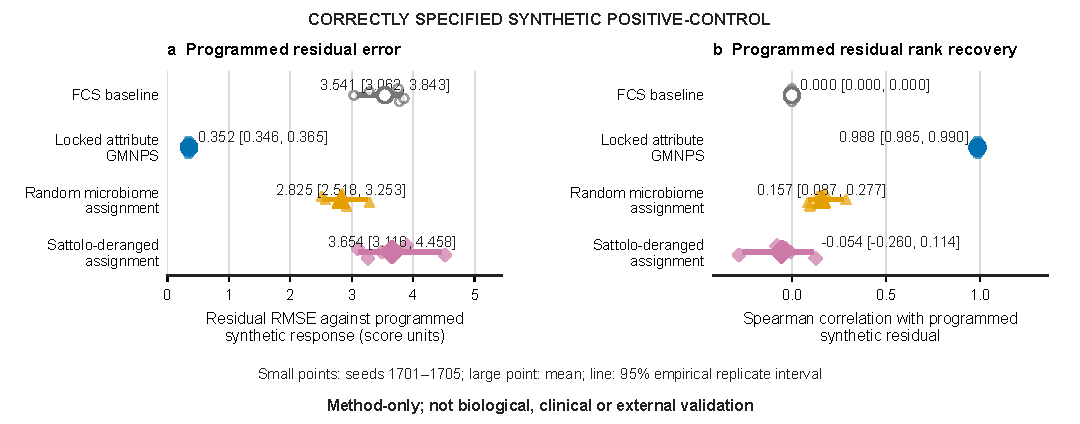
\includegraphics[width=\textwidth]{figures/supplementary_figure_S1_synthetic_positive_control.pdf}
\caption{\textbf{Correctly specified synthetic positive-control.}
\textbf{a}, Residual root-mean-square error against the programmed synthetic
response for the Food Compass baseline, locked attribute-level procedure,
random microbiome assignment and deterministic
Sattolo-deranged assignment. \textbf{b}, Spearman correlation between predicted
and programmed synthetic residuals for the same comparators. Small points
denote independent simulation seeds; large points and horizontal lines denote
the mean and empirical 2.5th--97.5th percentiles across five seeds. Each seed
comprised 24 synthetic individuals and 12 synthetic foods (288 person-food
pairs). The generator and evaluated code share the programmed mapping; the
controls belong to the same synthetic evidence family. The display assesses
numerical and assignment fidelity under correct specification only. Biological
misspecification was not assessed. Real
participant responses were not evaluated. External validity was not
established.}
\label{fig:supp_synthetic_positive_control}
\end{figure*}

Programmed-mapping recovery was lost after random or Sattolo-deranged
assignment. The random and deranged controls are parts of the same positive-
control family. The checks were fixed in the same code release and were not independently
preregistered. Because the generator uses the programmed mapping and domain
aggregation evaluated by the implementation, these findings test numerical and
assignment fidelity under correct specification. Biological misspecification
was not assessed. Real participant responses were not evaluated. External
validity was not established.

\subsection*{Combined evidence and expert-record boundary}

The fixed evidence decision remained at computational feasibility. No eligible
observed participant-by-meal outcome artifact, run-level method-lock instance,
paired metric table, prediction table, split audit or analysis-status artifact
was available. The production Food Compass and FNDDS registry also had no
approved artifact chain, and the supporting GMrepo, ZOE and knowledge-path
production registries or runs were absent.

\begin{table}[t]
\caption{\textbf{Combined evidence and expert-record boundary.} Missing
expert record classes are administrative author inputs and are not represented
as review outcomes.}
\label{tab:supp_evidence_expert_boundary}
\centering
\begin{tabular}{p{0.30\textwidth} p{0.22\textwidth} p{0.38\textwidth}}
\toprule
Evidence or record & Status & Authorized interpretation \\
\midrule
Locked attribute-level specification & Available & Computational method definition and invariants \\
Observed participant-by-meal outcomes & Unavailable & No direct-response or external-validity inference \\
Production 9,234-food run & Not executed & No population preservation, transition or heterogeneity inference \\
Correctly specified synthetic positive-control & Available & Implementation fidelity under programmed correct specification \\
Registry-bound GMrepo run & Not executed & No person-level generalization or disease result \\
Registry-bound ZOE rank run & Not executed & No aggregate rank-concordance result \\
Registry-bound knowledge-path run & Not executed & No biological or mechanistic validation result \\
External C1 feedback workbooks & Available and hash bound & Qualitative nutrient-channel content review \\
Anonymous item-level C3 records & AUTHOR\_INPUT\_NEEDED & No consensus percentage or final-passage claim \\
Anonymous item-level E4 records & AUTHOR\_INPUT\_NEEDED & No clinical-readiness or translation verdict \\
Exact reviewer denominator & Not established & No exact expert-count claim \\
\bottomrule
\end{tabular}
\end{table}

\subsection*{Available expert records supported content review only}

Available expert feedback informed the treatment of carbohydrate, zinc, copper
and vitamin A as retinol activity equivalents. The available evidence supports
qualitative content review only; the combined evidence and expert-record
boundary is reported in Supplementary Table S3.


\end{document}
